\section{Gold-Probe}\label{sec:gold}
Um den Umgang mit dem zur Verfügung stehenden RTM zu erlernen, wird zunächst eine Gold-Probe (Gold auf Saphir) untersucht, da hier die vorkommenden groben Strukturen leicht
abzubilden sind. In einem ersten Schritt wird eine Messspitze mit einem Seitenschneider aus dem Platin-Iridium-Draht zugeschnitten. Hier wird darauf geachtet,
dass der Platin-Iridium-Draht an einer Seite möglichst spitz zugeschnitten wird. Um eine Oberfläche mit atomarer Auflösung abzubilden, ist es notwendig, dass
die Spitze einatomig ist. Zuerst scheint es etwas unrealistisch, einen Draht auf eine einatomige Spitze zuzuschneiden. Allerdings wird es in der Praxis
meist der Fall sein, dass die zugeschnittene Spitze einatomig ist, da es immer ein Atom gibt, was im Vergleich zu seinem Nachbaratom noch ein wenig weiter vorne ist.
Dies reicht bereits für eine atomare Auflösung aus, da der Abstand zwischen Spitze und Probe in der Größenordnung eines Atomdurchmessers liegt. Somit wird
ein Elektron immer zu dem einzelnen vordersten Atom der Spitze tunneln, da die Tunnelwahrscheinlichkeit zu einem leicht dahinter liegenden Atom exponentiell
mit dem Abstand (bereits ungefähr zwei Atomdurchmesser) abfällt.\par
Die zugeschnittene Spitze kann nun in dem RTM-Innenleben zur Betrachtung unter der USB-Lupe befestigt werden. Diese Spitze wird für die gesamte Untersuchung
der Gold-Probe verwendet. In Abbildung \cref{fig:spitze1} ist die verwendete Spitze dargestellt. Links ist der Zustand der Spitze vor und rechts nach der Untersuchung
der Gold-Probe abgebildet. Der \SI{0,3}{\milli \meter}-dicke Platin-Iridium wird zur Kalibrierung der eingezeichneten Maßstäbe verwendet.
\begin{figure}[H]
    \centering
    \begin{subfigure}{0.45\textwidth}
        \centering
        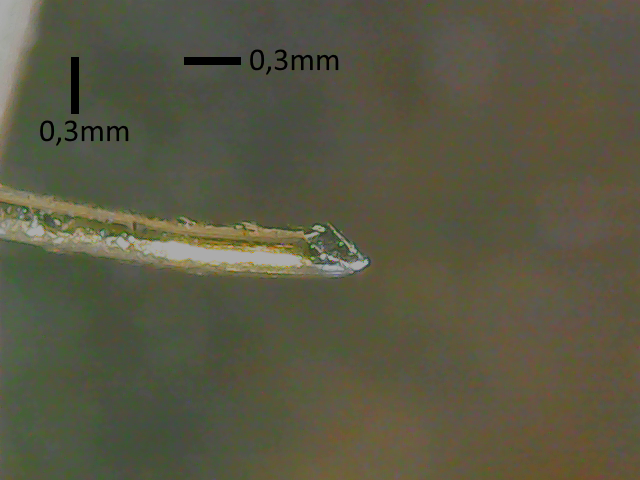
\includegraphics[width=\linewidth]{../figs/spitze1_vorher}
        \caption{vorher}
    \end{subfigure}
    \begin{subfigure}{0.45\textwidth}
        \centering
        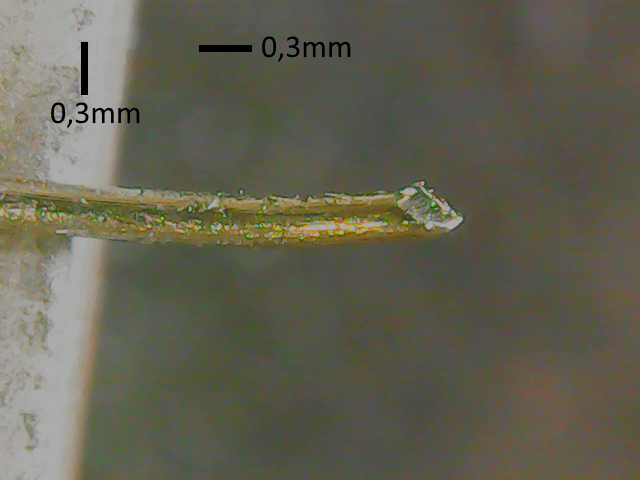
\includegraphics[width=\linewidth]{../figs/spitze1_nachher}
        \caption{nachher}
    \end{subfigure}
    \caption{Messspitze (Spitze 1) zur Untersuchung der Gold-Probe unter dem USB-Mikroskop}\label{fig:spitze1}
\end{figure} Mit dem USB-Mikroskop kann allerdings keine Aussage über die Qualität der Spitze getroffen werden. Es lässt sich auch nicht erkennen, ob
sich die Struktur der Spitze vorne während der Versuchsdurchführung maßgeblich verändert hat. Auch ist leider nicht zu erkennen, ob die Spitze
während der Versuchsdurchführung Dreck aufgesammelt hat, was unter anderem für schlechtere Messergebnisse gesorgt haben könnte.\par
Als Gold-Probe wird eine solche verwendet, bei der eine Goldschicht auf Saphir aufgetragen ist. Bevor diese Probe untersucht wird, wird
ihr Zustand mit dem USB-Mikroskop dokumentiert. Zur Kalibrierung des USB-Mikroskops wird ein $400 \times 100$-Mesh benutzt. Zur Kalibrierung werden
die \num{100} Mesh verwendet. Dies bedeutet, dass sich auf einem Zoll \num{100} Öffnungen befinden (vgl. \cite{mesh}). In \cref{fig:maßstab_gold} werden fünf solcher
Öffnungen abgezählt, womit die eingezeichnete Länge $\frac{5}{100} = \num{0,05}$ Zoll entspricht. Die Umrechnung in \unit{\milli \meter} wird durch eine
Multiplikation mit dem Faktor \num{25,4} vorgenommen (siehe \cite{umrechnung}). Die verwendete Gold-Probe ist in \cref{fig:gold_saphir} dokumentiert.
Der zuvor erstellte Maßstab wird mithilfe eines Bildbearbeitungsprogramms in das Bild der Gold-Probe übertragen. Auf der Gold-Probe sind einige Kratzer
aber auch einige augenscheinlich flache Stellen zu erkennen.\par
Nun werden Spitze und Probe in das RTM eingebaut. Der Annäherungsprozess erfolgt wie in \cref{sec:versuch} beschrieben. Nach einem erfolgreichen
Annäherungsprozess wird ein Tunnelstrom gemessen und die Rasterung der Oberfläche kann beginnen. Die Rasterung der Gold-Oberfläche wird ausschließlich
im \textit{constant-current-mode} vorgenommen, da die Gold-Probe eine raue und ungleichmäßige Oberfläche aufweist. So wird verhindert, dass die
Spitze in die Probe fährt. Nun können Bilder der Oberfläche der Goldprobe in verschiedenen Bildgrößen aufgenommen werden. Bei der Versuchsdurchführung
wurden auch häufig während einer Rasterungs-Periode die Programm-Parameter geändert, wodurch einige misslungene Bilder entstanden sind. Um auch generell
den Rahmen der Diskussion nicht zu sprengen, werden hier nur einige der gelungenen Bilder diskutiert. Alle aufgenommenen Bilder der
Gold-Probe sind in \url{https://uni-bonn.sciebo.de/s/wz3neQLAKV4slns} hinterlegt.
\begin{figure}[H]
	\centering
	\includegraphics[width=0.6\linewidth]{../figs/maßstab_gold.png}
	\caption{$400 \times 100$-Mesh zur Kalibrierung des Maßstabes des USB-Mikroskops}
	\label{fig:maßstab_gold}
\end{figure}
\begin{figure}[H]
	\centering
	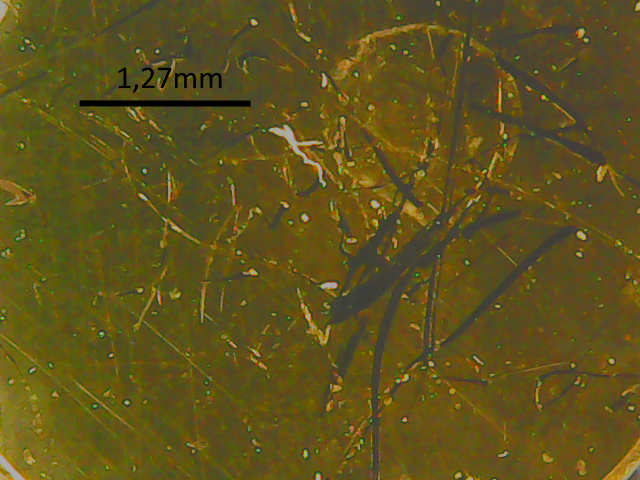
\includegraphics[width=0.6\linewidth]{../figs/gold_saphir.png}
	\caption{Mit dem USB-Mikroskop aufgenommene Oberfläche der verwendeten Gold-Probe (Goldschicht auf Saphir)}
	\label{fig:gold_saphir}
\end{figure}
Zunächst wird ein Bildausschnitt der Größe $\SI{200}{\nano \meter} \times \SI{200}{\nano \meter}$ ausgewählt, woraufhin einige Bilder aufgenommen werden.
Bei den aufgenommenen Bildern ist stets die sogenannte \textit{Time per line} hinterlegt, also in diesem Fall die Zeit, die die Spitze benötigt, um die Strecke
einer Linie (\SI{200}{\nano \meter}) zurückzulegen. Diese Größe lässt sich einfach in die tatsächliche Rastergeschwindigkeit umrechnen, indem die Länge einer Linie
durch die \textit{Time per line} geteilt wird. Die aufgenommenen Bilder werden mit der Software \texttt{Gwyddion} bearbeitet. Hier kann z.B. automatisch
ein Maßstab hinzugefügt werden. Außerdem wird die Farbgebung etwas geändert, sodass die Höhenunterschiede besser zu erkennen sind. In \cref{fig:gold1}
sind einige der RTM-Aufnahmen der Gold-Probe der Bildgröße \SI{200}{\nano \meter} dargestellt. Es ist sofort zu erkennen, dass die Gold-Oberfläche tatsächlich
sehr rau ist, da hier Höhenunterschiede in der Größenordnung von bis zu \SI{30}{\nano \meter} zu erkennen sind. Hier können jedoch nicht zwangsläufig Rückschlüsse
auf die Oberflächentopographie der Gold-Probe getroffen werden, da hier mit dem RTM im Wesentlichen die Elektronenverteilung (welche den Tunnelstrom verursacht) gemessen wird.
Gold ist ein Leiter, weshalb die Elektronen frei beweglich und delokalisiert sind. Dennoch ist es aus diesem Grund besonders einfach, gelungene Bilder
der Gold-Probe zu erzielen.
\begin{figure}[H]
    \centering
    \begin{subfigure}{0.45\textwidth}
        \centering
        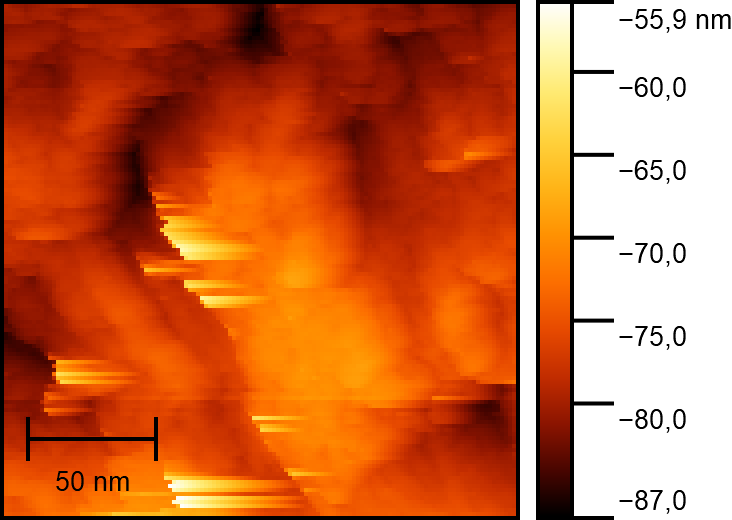
\includegraphics[width=\linewidth]{../figs/Gold10445}
        \caption{}
    \end{subfigure}
    \begin{subfigure}{0.45\textwidth}
        \centering
        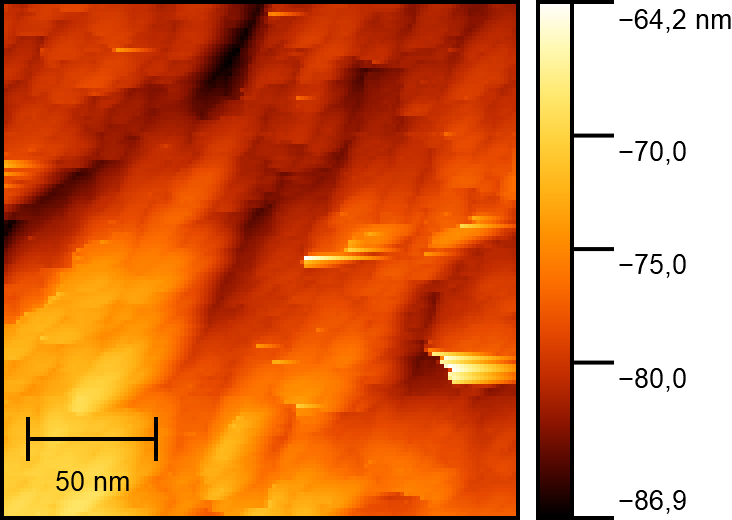
\includegraphics[width=\linewidth]{../figs/Gold10446}
        \caption{}
    \end{subfigure}
    \begin{subfigure}{0.45\textwidth}
        \centering
        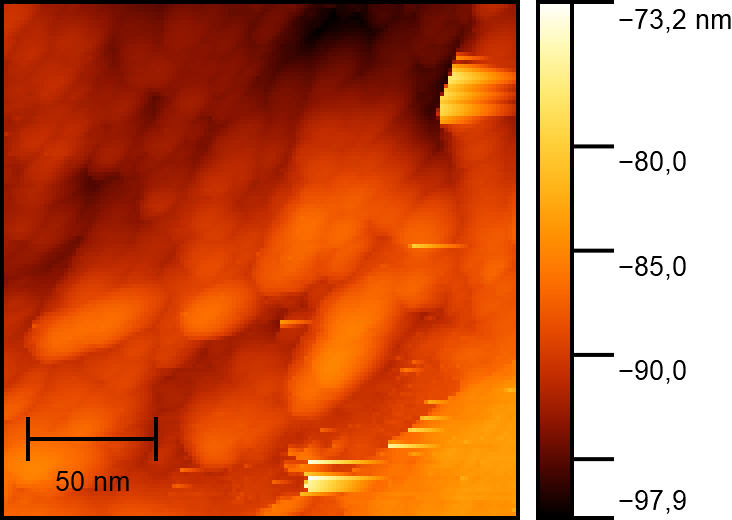
\includegraphics[width=\linewidth]{../figs/Gold10448}
        \caption{}
    \end{subfigure}
    \begin{subfigure}{0.45\textwidth}
        \centering
        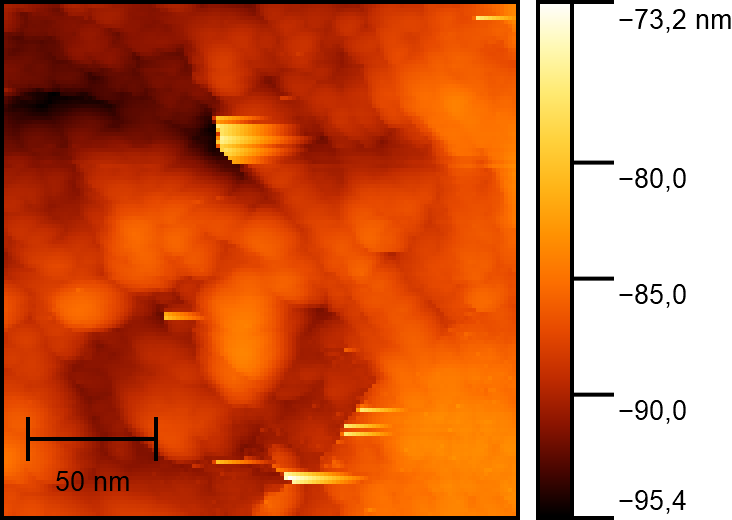
\includegraphics[width=\linewidth]{../figs/Gold10449}
        \caption{}
    \end{subfigure}
    \caption{RTM-Aufnahmen der Goldprobe. \textit{Image size} \SI{200}{\nano \meter}, \textit{Rastergeschwindigkeit} \SI{1e-6}{\meter \per \second}, \textit{Setpoint} \SI{1}{\nano \ampere},
    \textit{Tip voltage} \SI{1}{\volt}, \textit{P-Gain} \num{1000}, \textit{I-Gain} \num{2000}, \textit{D-Gain} \num{0}, Spitze 1}\label{fig:gold1}
\end{figure}
Die lokale Veränderung der Elektronenverteilung äußert sich in \cref{fig:gold1} darin, dass ständig der gleiche Ausschnitt der Gold-Probe betrachtet wird,
die resultierenden Bilder jedoch unterscheidbar sind. Ein weiterer Grund für die unterschiedlichen Bilder des gleichen Probenausschnitts lassen sich auch
durch einen Temperatur-Drift erklären. In dem Versuchsraum kommt es ständig zu Änderungen der Temperatur (z.B. durch die Anwesenheit/Abwesenheit von Menschen),
wodurch sich die Probe ausdehnt/zusammenzieht, was den betrachteten Bildausschnitt leicht verändert. Temperaturänderungen tragen auch zu Änderungen
der elektrischen Leitfähigkeit der Gold-Probe bei. Dennoch konnten hier gelungene Bilder der Gold-Probe aufgezeichnet werden. Es ist eine
wolkenartige Struktur zu erkennen. Diese Wolken scheinen sich wiederum aus kleinen Goldkugeln zusammenzusetzen, welche hier aber noch nicht
scharf genug aufgelöst sind. Außerdem sind mehrere sehr helle Punkte/Streifen zu erkennen, was darauf hindeutet, dass die Höhe der Spitze über der Probe aufgrund
eines plötzlichen hohen Tunnelstroms verändert werden musste. Die Ursache hierfür könnten kleine Verunreinigungen auf der Spitze oder auf der Probe sein.\par
Nun wird ein etwas kleinerer Bildausschnitt der Größe $\SI{84}{\nano \meter} \times \SI{84}{\nano \meter}$ ausgewählt, um die Struktur der kleinen Goldkugeln
besser auflösen zu können. Zwei der resultierenden Bilder sind in \cref{fig:gold2} dargestellt. Hierbei wurde auch mit verschiedenen Rastergeschwindigkeiten
und Werten für das \textit{I-Gain} experimentiert. Für die darauffolgenden Aufnahmen wurde jedoch der Wert für das \textit{I-Gain} wieder auf \num{2000} gestellt, da
die damit resultierenden Bilder meist besser aussahen. In \cref{fig:gold2} sind tatsächlich die Goldkugeln wesentlich besser zu erkennen. Viele von diesen
Goldkugeln sind etwa in der Größenordnung von \SI{10}{\nano \meter} bis \SI{30}{\nano \meter}, weshalb es sich hier auf keinen Fall um Goldatome sondern um Goldkugeln bestehend aus sehr
vielen Goldatomen handelt. Eine atomare Auflösung bei dieser Goldprobe ist aufgrund der hohen elektrischen Leitfähigkeit ohnehin nicht möglich. Um den Umgang
mit dem RTM etwas zu üben, wurde die Probe nun mit \textit{Withdraw} und \textit{Retract} von der Spitze entfernt. Dann wurde die Probe gleicht gedreht, um
einen anderen Ausschnitt der Oberfläche zu untersuchen. Mit \textit{Advance} und \textit{Approach} wurde die Probe dann wieder an die Spitze angenähert, was
erneut ohne Probleme funktionierte.
\begin{figure}[H]
    \centering
    \begin{subfigure}{0.45\textwidth}
        \centering
        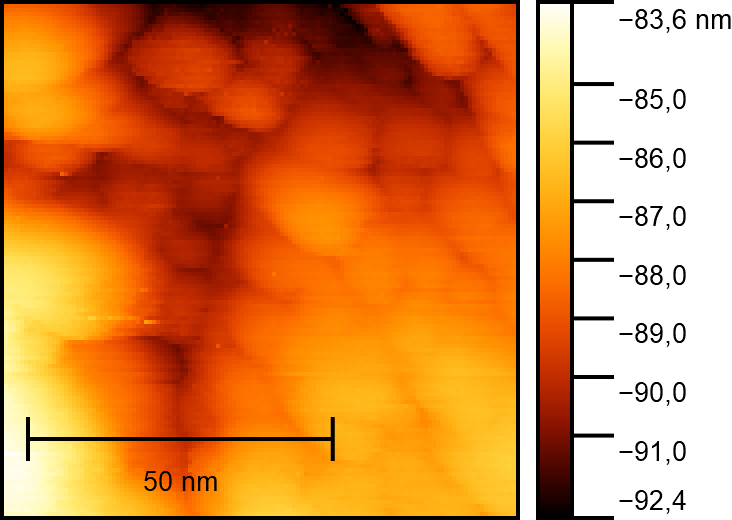
\includegraphics[width=\linewidth]{../figs/Gold10453}
        \caption{\textit{Rastergeschwindigkeit} \SI{4,2e-7}{\meter \per \second},\\ \textit{I-Gain} \num{2000}}
    \end{subfigure}
    \begin{subfigure}{0.45\textwidth}
        \centering
        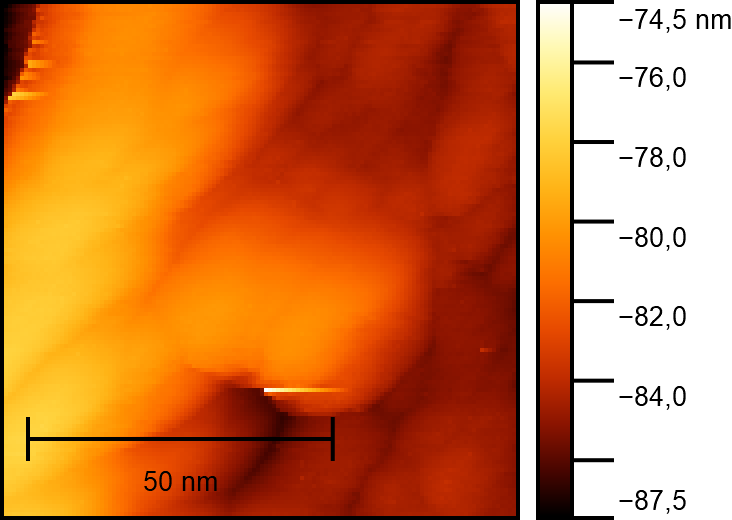
\includegraphics[width=\linewidth]{../figs/Gold10460}
        \caption{\textit{Rastergeschwindigkeit} \SI{8,4e-7}{\meter \per \second},\\ \textit{I-Gain} \num{2500}}
    \end{subfigure}
    \caption{RTM-Aufnahmen der Goldprobe. \textit{Image size} \SI{84}{\nano \meter}, \textit{Setpoint} \SI{1}{\nano \ampere},
    \textit{Tip voltage} \SI{500}{\milli \volt}, \textit{P-Gain} \num{1000}, \textit{D-Gain} \num{0}, Spitze 1}\label{fig:gold2}
\end{figure}
Erneut wird ein Bildausschnitt der Größe $\SI{200}{\nano \meter} \times \SI{200}{\nano \meter}$ ausgewählt. Das resultierende Bild ist in \cref{fig:gold3}
dargestellt. Im Vergleich zu \cref{fig:gold1} sind hier keine neuen Auffälligkeiten zu beobachten.
\begin{figure}[H]
	\centering
	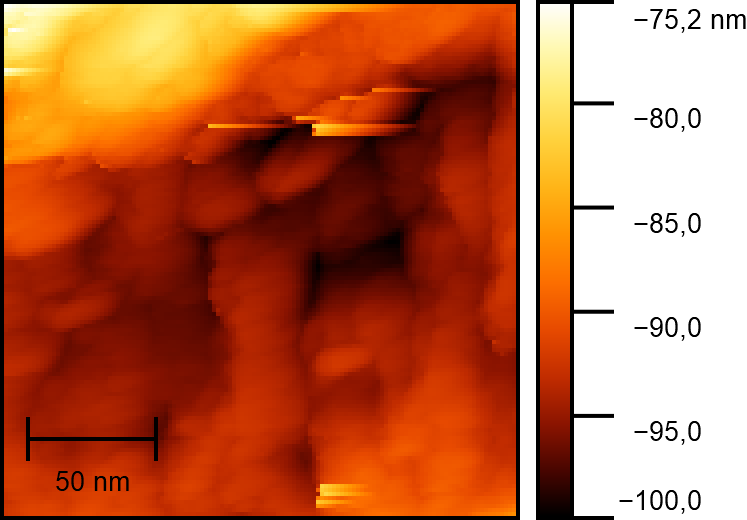
\includegraphics[width=0.6\linewidth]{../figs/Gold10468.png}
	\caption{RTM-Aufnahme der Goldprobe. \textit{Image size} \SI{200}{\nano \meter}, \textit{Rastergeschwindigkeit} \SI{1e-6}{\meter \per \second}, \textit{Setpoint} \SI{1}{\nano \ampere},
    \textit{Tip voltage} \SI{500}{\milli \volt}, \textit{P-Gain} \num{1000}, \textit{I-Gain} \num{2000}, \textit{D-Gain} \num{0}, Spitze 1}
	\label{fig:gold3}
\end{figure} Nun werden einige Bilder der Größe $\SI{50}{\nano \meter} \times \SI{50}{\nano \meter}$ aufgenommen (siehe \cref{fig:gold4}). Hier sind nun die einzelnen Goldkugeln
besser zu erkennen (zumindest in dem linken Bild). Das rechte Bild ist entweder sehr unscharf (was evtl. an einer zu hohen \textit{Tip voltage} liegt) oder in diesem Bildausschnitt
ist die Elektronenverteilung zum Zeitpunkt der Aufnahme etwas gleichmäßiger verteilt.\par
In \cref{fig:gold5} sind Bilder eines noch kleineren Bildausschnittes ($\SI{20}{\nano \meter} \times \SI{20}{\nano \meter}$) dargestellt. In dem linken Bild sind kaum noch Strukturen der
Goldoberfläche zu erkennen, die visuell getrennt werden können. In dem rechten Bild ist jedoch eine Abgrenzung von wahrscheinlich zwei Goldkugeln zu erkennen.\par
Abschließend sind in \cref{fig:gold6} Bilder eines sehr kleinen Ausschnittes ($\SI{5}{\nano \meter} \times \SI{5}{\nano \meter}$) gezeigt. Auf dieser Größenskala
können kaum noch differenzierte Strukturen aufgelöst werden, was durch die delokalisierte Elektronenverteilung zu begründen ist. Lediglich in dem rechten Bild ist eine leichte
Abgrenzung von zwei Strukturen zu erkennen, wobei hier aufgepasst werden muss, da die visuelle Darstellung trügen kann. Wie zu sehen ist, sind hier Höhenunterschiede
von nur \SI{2}{\nano \meter} vorhanden, weshalb es sich unter Umständen sogar um die gleiche Struktur handeln kann. Nun sind die Experimentierenden im Umgang mit dem RTM vertraut und
es kann die HOPG-Probe untersucht werden.
\begin{figure}[H]
    \centering
    \begin{subfigure}{0.45\textwidth}
        \centering
        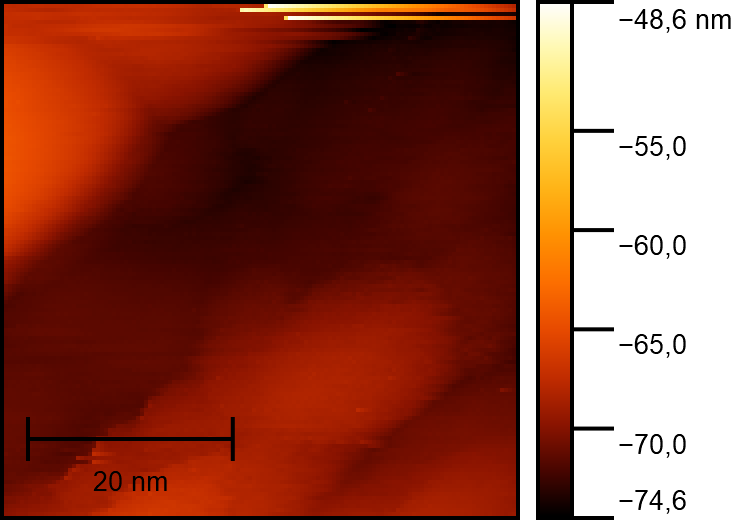
\includegraphics[width=\linewidth]{../figs/Gold10476}
        \caption{\textit{Tip voltage} \SI{200}{\milli \volt}}
    \end{subfigure}
    \begin{subfigure}{0.45\textwidth}
        \centering
        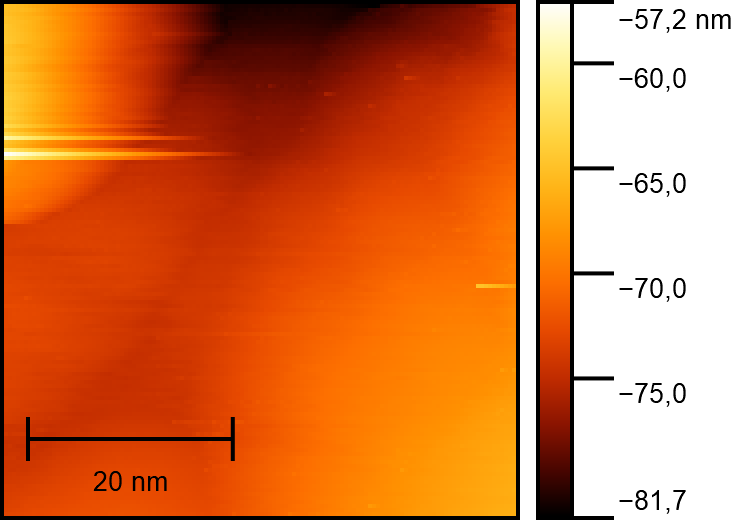
\includegraphics[width=\linewidth]{../figs/Gold10479}
        \caption{\textit{Tip voltage} \SI{1}{\volt}}
    \end{subfigure}
    \caption{RTM-Aufnahmen der Goldprobe. \textit{Image size} \SI{50}{\nano \meter}, \textit{Rastergeschwindigkeit} \SI{5e-7}{\meter \per \second}, \textit{Setpoint} \SI{1}{\nano \ampere},
    \textit{P-Gain} \num{1000}, \textit{I-Gain} \num{2000}, \textit{D-Gain} \num{0}, Spitze 1}\label{fig:gold4}
\end{figure}
\begin{figure}[H]
    \centering
    \begin{subfigure}{0.45\textwidth}
        \centering
        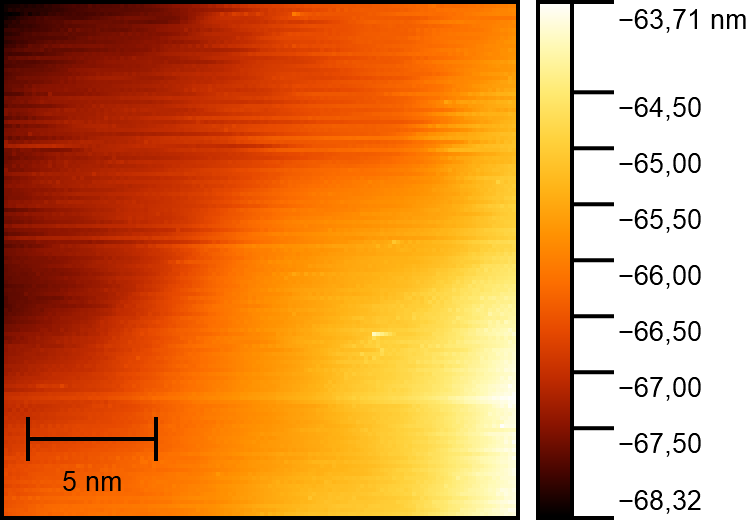
\includegraphics[width=\linewidth]{../figs/Gold10483}
        \caption{\textit{Rastergeschwindigkeit} \SI{4e-7}{\meter \per \second},\\ \textit{Tip voltage} \SI{200}{\milli \volt}}
    \end{subfigure}
    \begin{subfigure}{0.45\textwidth}
        \centering
        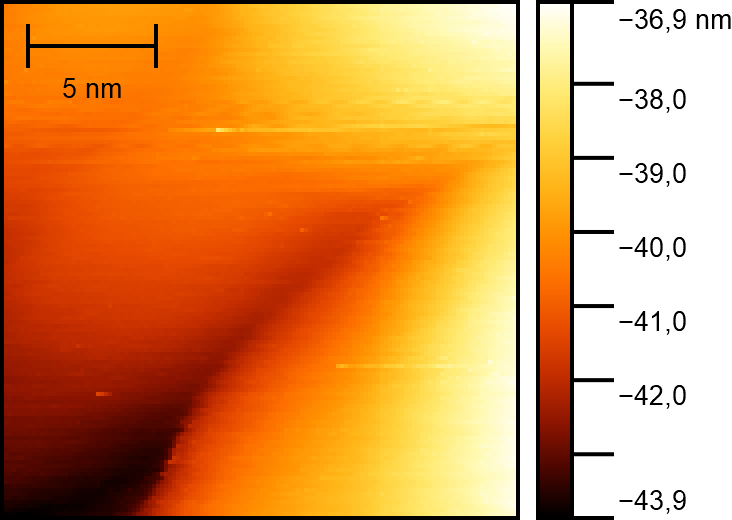
\includegraphics[width=\linewidth]{../figs/Gold10490}
        \caption{\textit{Rastergeschwindigkeit} \SI{2e-7}{\meter \per \second},\\ \textit{Tip voltage} \SI{1}{\volt}}
    \end{subfigure}
    \caption{RTM-Aufnahmen der Goldprobe. \textit{Image size} \SI{20}{\nano \meter}, \textit{Setpoint} \SI{1}{\nano \ampere},
    \textit{P-Gain} \num{1000}, \textit{I-Gain} \num{2000}, \textit{D-Gain} \num{0}, Spitze 1}\label{fig:gold5}
\end{figure}
\begin{figure}[H]
    \centering
    \begin{subfigure}{0.45\textwidth}
        \centering
        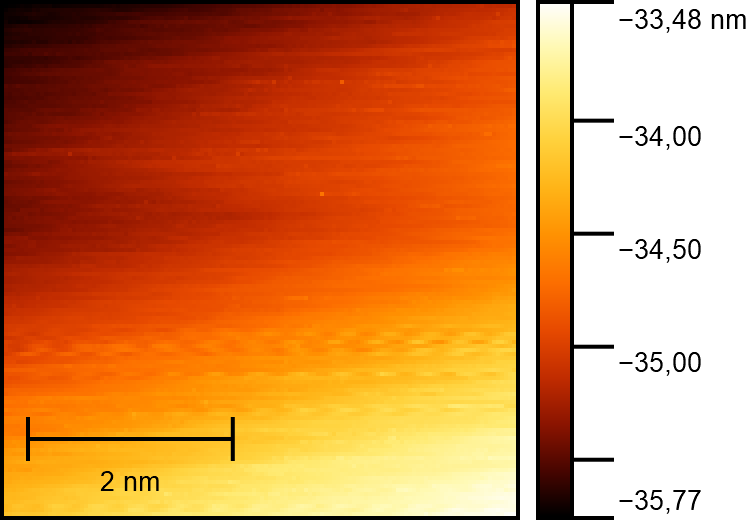
\includegraphics[width=\linewidth]{../figs/Gold10494}
        \caption{}
    \end{subfigure}
    \begin{subfigure}{0.45\textwidth}
        \centering
        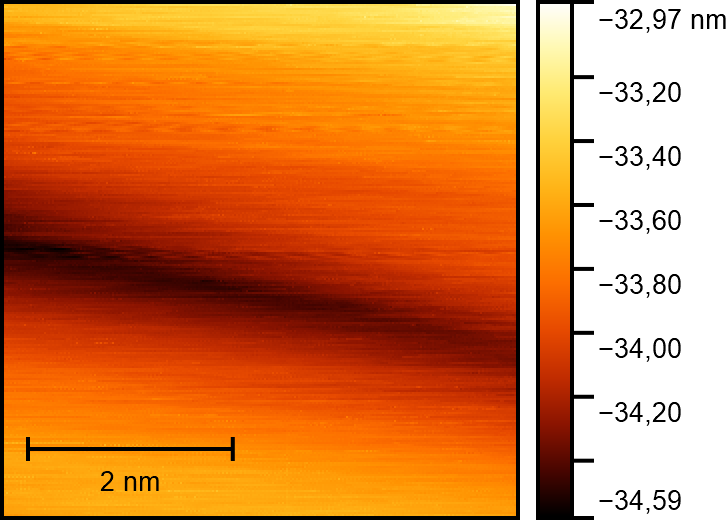
\includegraphics[width=\linewidth]{../figs/Gold10495}
        \caption{}
    \end{subfigure}
    \caption{RTM-Aufnahmen der Goldprobe. \textit{Image size} \SI{5}{\nano \meter}, \textit{Rastergeschwindigkeit} \SI{5e-8}{\meter \per \second}, \textit{Setpoint} \SI{1}{\nano \ampere},
    \textit{Tip voltage} \SI{500}{\milli \volt}, \textit{P-Gain} \num{1000}, \textit{I-Gain} \num{2000}, \textit{D-Gain} \num{0}, Spitze 1}\label{fig:gold6}
\end{figure}